\chapter{Markov Chains}
\newcommand*{\MC}{Markov Chains}
Bernoulli and Poisson process are memoryless and future outcomes do not depend on past. In the models we consider here, past has bearing on the future and therefore the model changes state with transition probabilities between states.

\section{Discrete-time Markov Chains}
The state changes at certain discrete time instants, indexed by an integer variable $n$. At each time step $n$, the state is denoted by $X_n$.

\begin{definition}[State space]
    The set of possible states of the model. We assume finite set of states $\mathcal S =\{1,\dots,m\}$.
\end{definition}
\begin{definition}[Transition probabilities $p_{ij}$]
    Whenever state happens to be $i$, there is probability $p_{ij}$ that the next state is equal to $j$.
    \[p_{ij}=\Pr(X_{n+1}=j|X_n=i). \quad i,j \in \mathcal{S}\]
\end{definition}

\subsubsection{Properties of transition probabilities are}
\begin{itemize}
    \item They are independent of the past and how state $i$ is reached.
    \[\Pr(X_{n+1}=j|X_n=i, X_{n-1}, \ldots, X_{0})=\Pr(X_{n+1}=j|X_n=i)=p_{ij}\]
    This is true at all times, for all states and for all sequences of past states.
    \item The transition probabilities are non-negative and sum to one.
    \[\sum_{j=0}^m p_{ij}=1, \quad \forall i\]
\end{itemize}

\begin{remark}
    In some cases where there is a dependence in the previous states, we can encode the dependency by changing the states in a way to eliminate the dependency.
\end{remark}
\subsection{Probability of a path}
Given a \MC we can compute the probability of any sequences of states by using multiplication rule.
\begin{align*}
    \Pr(X_0=i_0,X_1=i_1,\ldots,X_n=i_n) &= \Pr(X_n|X_1=i_1,\ldots,X_{n-1}=i_{n-1})\Pr(X_1=i_1,\ldots,X_{n-1}=i_{n-1}) \\
    &= \Pr(X_n|X_n=i_{n-1})\Pr(X_1=i_1,\ldots,X_{n-1}= i_{n-1}) \\
    &= p_{i_{n-1} n}\Pr(X_1=i_1,\ldots,X_{n-1}=i_{n-1}) \\
    &= p_{i_{n-1}n} \ldots p_{i_0i_1} \Pr(X_0=i_0)
\end{align*}

\subsection{$n$-step Transition Probabilities}
$r_{ij}(n)$ is the probability that the state after $n$ time periods will be $j$, given that the current state is $i$. It can be calculated using the following basic recursion, known as the Chapman-Kolmogorov equation.
\[r_{ij}(n)=\begin{cases}
    \sum_{k=1}^{m}r_{ik}(n-1)p_{kj} & \quad n>1 \\
    p_{ij} & \text{n=1}
\end{cases}\]

\section{Classification of States}
We now classify states based on their long-term frequency with which they are visited.

\begin{definition}[Accessible]
    A state $j$ is accessible from state $i$ iff $r_{ij}(n)$ is positive. In other words, there is a path $i,i_1,\ldots,i_{n-1},j$ which starts at $i$ and ends at $j$, in which the transitions $(i,i_1), (i_1,i_2), \ldots, (i_{n-1},j)$ have positive probability.
\end{definition}
Let $A(i)$ be the set of states accessible from $i$. For a recurrent state $i$, $A(i)$ is called as a recurrent class.
\begin{definition}[Recurrent]
    State $i$ is recurrent if for every state $j\in A(i)$ we have $i \in A(j)$. That is, the set of states which are accessible from each other are called as recurrent.
\end{definition}
\begin{remark}
    A set of recurrent states form a strongly connected component.
\end{remark}
\begin{definition}[Transient]
    A state which is not recurrent.
\end{definition}
A transient state can be visited only a finite number of times because every time you visit that state there is a positive probability of reaching a state from which there is no coming back. This is not the case with recurrent state.

There must exist at least one recurrent class.

\subsection{Periodicity}
A recurrent class is called periodic if it can be decomposed into $d>1$ disjoint subsets $S_1,\ldots,S_d$ so that all transitions from one subset lead to next subset.
\[\text{if } i\in S_k \text{ and } p_{ij}>0, \quad \text{then } \begin{cases}
    S_{k+1} & k=1,\ldots, d-1 \\
    S_1 & k=d
\end{cases}\]

For a periodic recurrent class $R$ at a given positive time $n$ and state $i$ there exists one or more states with $r_{ij}(n)=0$. Thus starting from a state $i$ only a set of states are accessible at a given time. 

This gives us a way to test aperiodicity. If there is a special time $n\ge 1$ and a special state $i\in R$ from which all states in $R$ can be reached then $R$ is aperiodic. Converse is also true if $R$ is aperiodic then there exists a time $n$ such that $r_{ij}(n)>0, \forall i,j \in R$.

\section{Steady-State Behavior}
We're interested in values of $r_{ij}(n)$ when $n$ is very large. If there are more than one recurrent classes then the limiting values of $r_{ij}(n)$ depends on the initial state. So we'll restrict us with a single recurrent class plus some transient states.
\begin{remark}
    The asymptotic behavior of a multiclass chain can be understood in terms of the asymptotic behavior of a single-class chain.
\end{remark}
The conditions required for steady state values are
\begin{enumerate}
    \item Single recurrent class
    \item Aperiodicity
\end{enumerate}
Therefore we can have limiting probabilities $\pi_j$ of ending up in state $j$ independent of initial state after a long time.
\[\pi_j\approx \Pr(X_n=j), \quad \text{when } n \text{ is large}\]

\begin{theorem}[Steady-State convergence]
    Consider a Markov chain with a single recurrent class, which is aperiodic. Then, the states j are associated with steady-state probabilities $\pi_{j}$ that have the following properties.
    \begin{enumerate}
        \item For each $j$, we have 
        \[\lim_{n\to \infty} r_{ij}(n)=\pi_j, \quad \forall i\]
        \item The $\pi_j$ are the unique solution to the balance equations
        \begin{align*}
            \pi_j &= \sum_{k=1}^m \pi_k p{kj}, \quad, j=1,
            \ldots, m\\
            1 &= \sum_{k=1}^m \pi_k
        \end{align*}
        \item We have \[\pi_j \begin{cases}
            =0 & \text{ for all transient states }j \\
            >0 & \text{ for all recurrent states }j
        \end{cases}\]
    \end{enumerate}
\end{theorem}

\subsection{Long-Term Frequency Interpretations}

We can interpret the steady-state probabilities in terms of expected state frequencies.

For a Markov chain with a single class which is aperiodic, the steady-state probabilities $\pi_j$ satisfy
\[\pi_j=\lim_{n\to \infty}\frac{v_{ij}(n)}{n}\]

where $v_{ij}$ is the expected number of visits starting to state $j$ starting from state $i$.

Let $q_{jk}(n)$ be the expected number of transitions that take the state from $j$ to $k$. Then regardless of the initial state
\[\lim_{n \to \infty}\frac{q_{jk}(n)}{n}=\pi_j p_{jk}\]

Using the above interpretations the balance equation make sense intuitively
\[\sum_{k=1}^m\pi_k p_{kj}=pi_j\]
because the expected frequency $\pi_j$ of visits to $j$ is the sum of expected frequencies $\pi_k p_{kj}$ of transitions that lead to $j$.

\begin{figure}[!h]
    \centering
    \begin{center}


    \tikzset{every picture/.style={line width=0.75pt}} %set default line width to 0.75pt        

    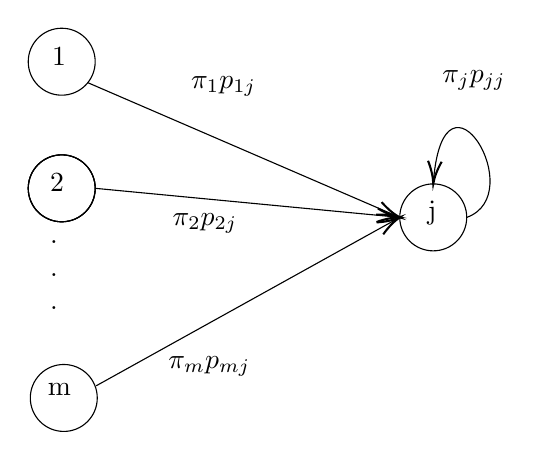
\begin{tikzpicture}[x=0.75pt,y=0.75pt,yscale=-1,xscale=1]
    %uncomment if require: \path (0,300); %set diagram left start at 0, and has height of 300
    
    %Shape: Circle [id:dp1080866293664855] 
    \draw   (168.74,89.13) .. controls (168.74,80.22) and (175.96,73) .. (184.87,73) .. controls (193.78,73) and (201,80.22) .. (201,89.13) .. controls (201,98.04) and (193.78,105.26) .. (184.87,105.26) .. controls (175.96,105.26) and (168.74,98.04) .. (168.74,89.13) -- cycle ;
    %Shape: Circle [id:dp8469939459955591] 
    \draw   (168.74,150.13) .. controls (168.74,141.22) and (175.96,134) .. (184.87,134) .. controls (193.78,134) and (201,141.22) .. (201,150.13) .. controls (201,159.04) and (193.78,166.26) .. (184.87,166.26) .. controls (175.96,166.26) and (168.74,159.04) .. (168.74,150.13) -- cycle ;
    %Shape: Circle [id:dp5676474110088898] 
    \draw   (168.74,150.13) .. controls (168.74,141.22) and (175.96,134) .. (184.87,134) .. controls (193.78,134) and (201,141.22) .. (201,150.13) .. controls (201,159.04) and (193.78,166.26) .. (184.87,166.26) .. controls (175.96,166.26) and (168.74,159.04) .. (168.74,150.13) -- cycle ;
    %Shape: Circle [id:dp9671873474577539] 
    \draw   (168.74,150.13) .. controls (168.74,141.22) and (175.96,134) .. (184.87,134) .. controls (193.78,134) and (201,141.22) .. (201,150.13) .. controls (201,159.04) and (193.78,166.26) .. (184.87,166.26) .. controls (175.96,166.26) and (168.74,159.04) .. (168.74,150.13) -- cycle ;
    %Shape: Circle [id:dp997416844792204] 
    \draw   (169.74,251.13) .. controls (169.74,242.22) and (176.96,235) .. (185.87,235) .. controls (194.78,235) and (202,242.22) .. (202,251.13) .. controls (202,260.04) and (194.78,267.26) .. (185.87,267.26) .. controls (176.96,267.26) and (169.74,260.04) .. (169.74,251.13) -- cycle ;
    %Shape: Circle [id:dp9895222198724538] 
    \draw   (347.74,164.13) .. controls (347.74,155.22) and (354.96,148) .. (363.87,148) .. controls (372.78,148) and (380,155.22) .. (380,164.13) .. controls (380,173.04) and (372.78,180.26) .. (363.87,180.26) .. controls (354.96,180.26) and (347.74,173.04) .. (347.74,164.13) -- cycle ;
    %Straight Lines [id:da6194457169140921] 
    \draw    (197.51,99.26) -- (345.91,163.34) ;
    \draw [shift={(347.74,164.13)}, rotate = 203.35] [color={rgb, 255:red, 0; green, 0; blue, 0 }  ][line width=0.75]    (10.93,-3.29) .. controls (6.95,-1.4) and (3.31,-0.3) .. (0,0) .. controls (3.31,0.3) and (6.95,1.4) .. (10.93,3.29)   ;
    %Straight Lines [id:da4206665530374054] 
    \draw    (201,150.13) -- (345.75,163.94) ;
    \draw [shift={(347.74,164.13)}, rotate = 185.45] [color={rgb, 255:red, 0; green, 0; blue, 0 }  ][line width=0.75]    (10.93,-3.29) .. controls (6.95,-1.4) and (3.31,-0.3) .. (0,0) .. controls (3.31,0.3) and (6.95,1.4) .. (10.93,3.29)   ;
    %Straight Lines [id:da5931367337880484] 
    \draw    (201.51,245.26) -- (345.99,165.1) ;
    \draw [shift={(347.74,164.13)}, rotate = 510.98] [color={rgb, 255:red, 0; green, 0; blue, 0 }  ][line width=0.75]    (10.93,-3.29) .. controls (6.95,-1.4) and (3.31,-0.3) .. (0,0) .. controls (3.31,0.3) and (6.95,1.4) .. (10.93,3.29)   ;
    %Curve Lines [id:da05042747344345444] 
    \draw    (380,164.13) .. controls (410.69,153.24) and (369.35,84.65) .. (364.02,146.1) ;
    \draw [shift={(363.87,148)}, rotate = 274.1] [color={rgb, 255:red, 0; green, 0; blue, 0 }  ][line width=0.75]    (10.93,-3.29) .. controls (6.95,-1.4) and (3.31,-0.3) .. (0,0) .. controls (3.31,0.3) and (6.95,1.4) .. (10.93,3.29)   ;
    
    % Text Node
    \draw (179,81) node [anchor=north west][inner sep=0.75pt]   [align=left] {1};
    % Text Node
    \draw (178,142) node [anchor=north west][inner sep=0.75pt]   [align=left] {2};
    % Text Node
    \draw (177,242.99) node [anchor=north west][inner sep=0.75pt]  [font=\normalsize] [align=left] {m};
    % Text Node
    \draw (360,155) node [anchor=north west][inner sep=0.75pt]   [align=left] {j};
    % Text Node
    \draw (246,95) node [anchor=north west][inner sep=0.75pt]   [align=left] {$\displaystyle \pi _{1} p_{1j}$};
    % Text Node
    \draw (237,161) node [anchor=north west][inner sep=0.75pt]   [align=left] {$\displaystyle \pi _{2} p_{2j}$};
    % Text Node
    \draw (235,230) node [anchor=north west][inner sep=0.75pt]   [align=left] {$\displaystyle \pi _{m} p_{mj}$};
    % Text Node
    \draw (367,92) node [anchor=north west][inner sep=0.75pt]   [align=left] {$\displaystyle \pi _{j} p_{jj}$};
    % Text Node
    \draw (178,174) node [anchor=north west][inner sep=0.75pt]   [align=left] {.\\.\\.};
    
    
    \end{tikzpicture}
    
\end{center}

    \caption{Interpretation of balance equations}
 \end{figure}

\subsection{Birth-Death Process}
In these processes states are linearly arranged and transitions can only occur between neighboring states.
\begin{align*}
    b_i &= \Pr(X_{n+1}=i+1 | X_n=i) \\
    d_i &= \Pr(X_{n+1}=i-1 | X_n=i)
\end{align*}

\begin{figure}[!h]
   \centering
   \includegraphics[width=.6\textwidth]{images/P_Markov_Birth_Death.png}
   \caption{Transition probability graph for a birth-death process}
\end{figure}

For two neighboring states $i, i+1$. For another transition of $i \to i+1$ can occur there must a transition of $i+1 \to i$. Therefore expected frequency of transitions satisfies
\[\pi_i b_i=\pi_{i+1}d_{i+1}, \quad i=0,1,\ldots,m-1\]
This leads us to local balance equations
\begin{align*}
    \pi_i &= \pi_0 \frac{b_0 b_1 \cdots b_{i-1}}{d_1 d_2 d_i}, \quad i=1,2,\cdots, m \\
    \sum_i \pi_i &= 1
\end{align*}

\begin{remark}
    Consider the case where $m$ is very large and $b>d$ the steady state probability of all states will be zero and it will be transient. Thus even with aperiodic single recurrent class a \MC{} may fail to reach steady state values and a steady-state distribution may not exist.
\end{remark}